\section{Diskussion}
Betrachtet man die Ergebnisse für den Fluss in Abbildung \ref{fig:Fluss} fällt auf, dass die beiden Entfaltungsmöglichkeiten zu einem nahezu identischem Ergebnis führen. Betrachtet man die Unsicherheiten bei der Likelihood-Entfaltung, fällt auf, dass gerade bei hohen Energien der Fluss große Unsicherheiten besitzt. In diesem Bereich ist der Untergrund extrem klein, aber (??).\\
\begin{figure}
	\begin{subfigure}[c]{0.5\textwidth}
		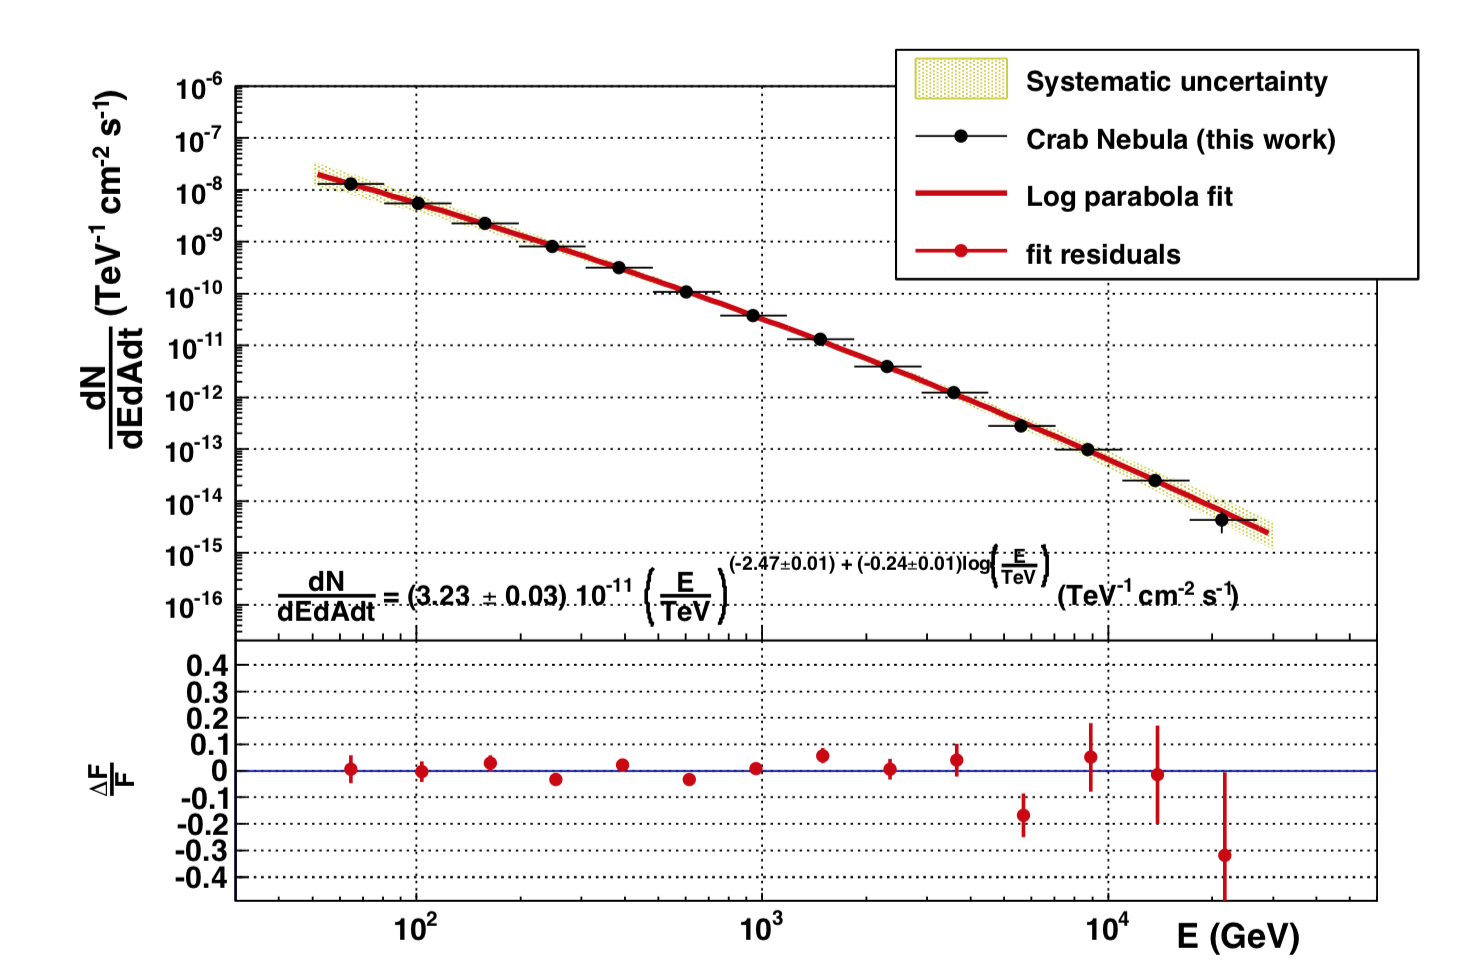
\includegraphics[width=\textwidth]{graphics/Magic.png}
		\subcaption{Der von der MAGIC Kolloboration bestimmte Fluss des Krebsnebels.\cite{Aleksic:2014jva}}
	\end{subfigure}
	\begin{subfigure}[c]{0.5\textwidth}
		\includegraphics[width=\textwidth]{plots/Fluss_Like.pdf}
		\subcaption{Der mit Likelihood-Entfaltung bestimmte Fluss des Krebsnebels.}
	\end{subfigure}
	\caption{Vergleich der Messungen zum Fluss des Krebsnebels mit MAGIC und FACT Daten.}
\end{figure}
Vergleicht man den berechneten Fluss aus der Entfaltung der FACT-Daten mit dem aus der Veröffentlichung \cite{Aleksic:2014jva} der MAGIC Kolloboration fällt auf, dass der Fluss nahezu in der selben größen Ordnung liegt. Der Fluss aus den FACT-Daten ist ein wenig geringer. Dies könnte an den unterschiedlichen Detektorsystemen liegen.
